\section{Floppy Controller}
\begin{figure}[h!]
    \centering
    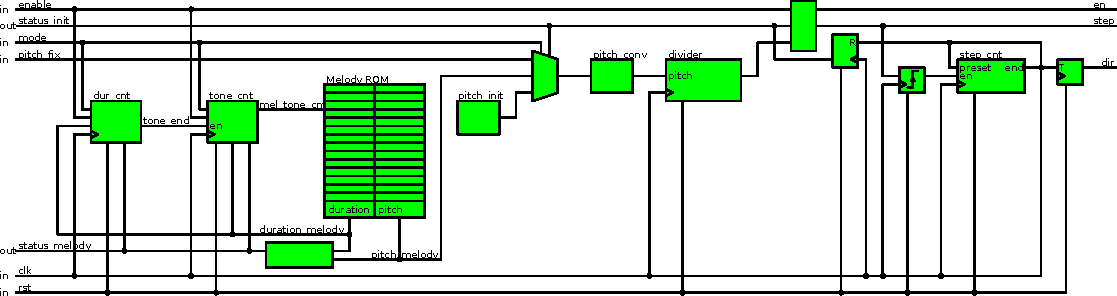
\includegraphics[width=1.0\textwidth]{../organization/floppy_controller.pdf}
    \caption{Blockschaltbild Floppy Peripherie Komponente}
    \label{fig:block}
\end{figure}
\noindent Der Floppy Controller steuert ein Diskettenlaufwerk an. Dazu werden die 
Signale Step und Dir generiert, welche den Schrittmotor für die 
Kopfpositionierung ansteuern. Nach 80 Schritten wird jeweils die Richtung der 
Kopfbewegung umgekehrt, damit der Lesekopf nicht am mechanischen Endanschlag 
ansteht. Nach dem Reset wird der Lesekopf um 80 Schritte in eine Richtung 
gefahren. Die Kopfposition wird dann vom Laufwerk mittels einer eingebauten 
Gabellichtschranke initialisiert. Anschliessend können Töne erzeugt werden. 
Als Quelle für die Töne kann einerseits das Signal \verb!pitch_fix! verwendet 
werden. Dazu muss das Signal \verb!mode! auf \verb!'0'! stehen. Die einzelnen 
Töne sind nummeriert. Die Nummerierung entspricht dabei der Nummerierung im 
MIDI\footnote{\textbf{M}usical \textbf{I}nstrument \textbf{D}igital 
\textbf{I}nterface} Standard (Siehe \autoref{tab:midi}). Liegt am Signal 
\verb!mode! \verb!'1'! an, so wird das Moduleigene Melody 
ROM\footnote{\textbf{R}ead \textbf{O}nly \textbf{M}emory} verwendet. Darin 
sind jeweils Tonhöhe und die Spieldauer des jeweiligen Tones in 
\si{\milli\second} abgelegt. Ist die Spieldauer des jeweiligen Tones 
abgelaufen, wird der nächste Ton geladen und abgespielt. Als Beispielmelodie 
ist Axel F von Harold Faltermeyer implementiert. 
\begin{table}[h!]
    \centering
    \begin{zebratabular}{ll}
        \rowcolor{gray} MIDI Nummer & Frequenz \\
         45 & 110   \si{\hertz} \\
         46 & 116.5 \si{\hertz} \\
         47 & 123.4 \si{\hertz} \\
         48 & 130.8 \si{\hertz} \\
         49 & 138.5 \si{\hertz} \\
         50 & 146.8 \si{\hertz} \\
         51 & 155.5 \si{\hertz} \\
         52 & 164.8 \si{\hertz} \\
         53 & 174.6 \si{\hertz} \\
         54 & 184.9 \si{\hertz} \\
         55 & 195.9 \si{\hertz} \\
         56 & 207.6 \si{\hertz} \\
         57 & 220   \si{\hertz} \\
         58 & 233.0 \si{\hertz} \\
         59 & 246.9 \si{\hertz} \\
         60 & 261.6 \si{\hertz} \\
         61 & 277.1 \si{\hertz} \\
         62 & 293.6 \si{\hertz} \\
         63 & 311.1 \si{\hertz} \\
         64 & 329.6 \si{\hertz} \\
         65 & 349.2 \si{\hertz} \\
         66 & 369.9 \si{\hertz} \\
         67 & 391.9 \si{\hertz} \\
         68 & 415.3 \si{\hertz} \\
         69 & 440   \si{\hertz} \\
         70 & 466.1 \si{\hertz} \\
    \end{zebratabular}
    \caption{Zuordung MIDI Nummer $\to$ Frequenz (Auszug)}
    \label{tab:midi}
\end{table}
